%! Author = lili
%! Date = 4/27/26


\chapter{Grenzwertsätze}\label{ch:grenzwertsatze}
\untit{Vorlesung 13. Juni 2025 (V09 2025) und 12. Juni 2026 (V08 2026)} % und 08 bzw 12 Juni in 2026
\section{Markoffsche und Tschebyscheffsche Ungleichung}
\begin{satz}
    \textbf{Markoffsche Ungleichung} \txc{(2026)} \\
    %  F 2
    Sei $X$ eine Zufallsvariable. $\E{|X|^k}$ existiert für ein $k \in \nz$.
    Dann existiert auch der Erwartungswert $\E{X}$, und es gilt
    \[
        \pe( \oub{|X - \E{X}|}{*} \geq h ) \leq \frac{\E{|X - \E{X}|^k}}{h^k} \quad \forall h > 0
    \]
    \txo{* Menge aller $\oio$ derart, dass $X(\ele)$ um mindestens h von ihrem EW $\E{X}$ abweicht.}
\end{satz}

\begin{satz}
    \textbf{Tschebyscheffsche Ungleichung (Spezialfall k = 2)} \txc{(2026)}  \\
    %  F 3
    Für eine Zufallsvariable X, deren Erwartungswert und Varianz existieren, gilt
    \[
        \pe( |X - \E{X}| \geq h ) \leq \frac{\Var(X)}{h^2} \quad \forall h > 0
    \]
    \paragraph{Beweis:} \txo{Spezialfall diskreter \glspl{wraum}}
    \begin{align*}
        \pe( |X - \E{X}| \geq h ) & = \sum_{\oio : |X(\ele)- \E{X}| \geq h} \wfk(\ele) \\
        & = \sum_{x \in X(\eraum) : |x - \E{X}| \geq h} \pe( \{\oio: X(\ele) = x\} ) \\
        & \leq  \sum_{x \in X(\eraum) : |x - \E{X}| \geq h} \big( \frac{|x - \E{X}|}{h} \big)^2 \pe(X=x) \\
        & \leq \frac{1}{h^2}  \sum_{x \in X(\eraum)} |x - \E{X}|^2  \pe(X=x)  \\
        & \leq  \frac{1}{h^2} \Var(X)
    \end{align*}
\end{satz}

\begin{bsp}
    \textbf{Die Tschebyscheffsche Ungleichung kann nicht verbessert werden} \txc{(2026)} \\
    %  F 4-9
    Sei $N \in \nz$ beliebig und die Zufallsvariable $X$ mit $X(\eraum) = \{ -N, 0, +N\}$ und $\pe ( X = \pm N) = \frac{1}{2N^2}$
    % TODO Ist X damit vollständig beschrieben?
    \begin{align*}
        \txo{\pe( X= +N)} & \txo{= \frac{1}{2N^2}} \\
        \txo{\pe( X= -N)} & \txo{= \frac{1}{2N^2}} \\
        \txo{\pe( X= 0)} & \txo{= 1- \frac{1}{N^2}}
    \end{align*}
    Aus $\E{X} = 0$ folgt
    \[
        \Var(X) = N^2 \pe (X = -N) + N^2 \pe (X = +N) = 1
    \]
    \txo{Denn}
    \[
        \txo{
        \Var(X) = \E{X^2} = N^2 \pe(X^2 = N) = N^2 \frac{2}{2N^2} = 1
        }
    \]
    Für jedes $h \in (0,N]$ gilt
    \begin{align*}
        \pe(|X - \oub{\E{X}}{=0}|  \geq h ) & =  \pe(|X - \E{X} | > 0) \\
        & = \pe (X = N) + \pe (X = -N) \\
        & = \frac{1}{N^2} \\
        & = \frac{ \oob{\Var(X)}{=1} }{N^2} \\
        & \leq \frac{1}{h^2} \Var(X)
    \end{align*}
    Die Wahl $h = N$ zeigt: Ungleichung kann nicht verbessert werden.

    Die Wahl $h = 2N$ dagegen zeigt, dass sie nicht immer gut ist:
    \[
        \pe(|X - \E{X} | \geq 2N) = \pe(|X | > N) = 0 < \frac{1}{(2N)^2} = \frac{\Var(X)}{(2N)^2}
    \]
\end{bsp}

\begin{bsp}
    \textbf{Werfen eines fairen Würfels} \txc{(2026)}\\
    % F 10 - 16
    Wie oft müssen wir einen fairen Würfel werfen, bis mit Ws. $\geq 1  - 0.05$ die relative Häufigkeit einer Sechs um weniger als 1/10 von 1/6 abweicht?
    \paragraph{Ansatz:} $\eraum = \{1, \dots, 6\}^N$ mit Gleichverteilung $\pe$ (für N Würfe) und Zufallsvariablen
    $X_i \eraum \rightarrow \{0,1\}$.

    Dabei sind $X_i(\ele) = 1_{\{6\}} (\ele_i)$ unabhängig und identisch verteilt (u.i.v.) mit $\pe(X_i = 1) = \frac{1}{6}$.

    $S_N = \sum^N_{i=1} X_i$ ist die Anzahl der geworfenen Sechsen und $\frac{1}{N} S_N$ ist die relative
    Häufigkeit einer Sechs.
    \paragraph{Gesucht} ist das kleinste N derart, dass $ \pe\left(| \frac{S_N}{N} - \frac{1}{6}| \geq \frac{1}{10}\right) \leq \frac{5}{100}$
    \txo{(Gegenereignis zu $\pe\left(| \frac{S_N}{N} - \frac{1}{6}| < \frac{1}{10}\right) \geq 1- \frac{5}{100}$ )}.
    \paragraph{Lösung:} \txo{für Tschebyscheffsche Ungleichung in Bezug auf EW und Var} \\
    Seien p = 1/6 und q = 1 - p = 5/6 und sei $S_N$ binomialverteilt mit Parametern N und p.
    Dann ist
    \[
        \E{ \frac{1}{N}  S_N} = \frac{1}{N} \E{S_N} \overset{\txc{*}}{=}  \frac{1}{N} Np  = p = 1/6
    \]
    \txc{* da $S_N$ binomialverteilt ist}
    und
    \[
        \Var\left(\frac{1}{N}  S_N\right) = \frac{1}{N} \Var(S_N) \overset{\txc{**}}{=} \frac{1}{N} Npq = \frac{1}{N} pq = \frac{1}{N} \frac{1}{6} \frac{5}{6}
    \]
    \txc{** Ebenfalls, weil $S_N$ binomialverteilt ist.} \\
    Tschebyscheffsche Ungleichung:
    \[
        \pe\left(
        \oub{
            | \frac{S_N}{N} - \frac{1}{6} | \geq \frac{1}{10}
        }{Gegenereignis}
        \right)
        \leq 
        \frac{\Var\left(\frac{S_N}{N}\right)}{(1/10)^2} = 100 \frac{5}{36 N}
    \]
    Wir wählen also N so groß, dass $100 \frac{5}{36 N} \leq \frac{5}{100}$.
    \paragraph{Fazit}
    Jedes $N \approx 278$ (genauer aus der Abschätzung $(100)^2/36 \approx 277.7$) garantiert, dass mit
    Wahrscheinlichkeit $\geq 0.95$ die relative Häufigkeit einer Sechs bei $N$-maligem Würfeln um weniger als $1/10$
    von $1/6$ abweicht.

    Wenn wir $N = 278$ wählen, sind wir auf der sicheren Seite.

    Da wir abgeschätzt haben, ist dieses $N$ möglicherweise nicht das minimale.
\end{bsp}

\karkar{satz_markoffsche_ungleichung}
\karkar{satz_tschebyscheffsche_ungleichung}
\karkar{bem_nutzen_tschebyscheff_ungleichung}
\karkar{bem_tschebyscheff_ungleichung_scharf}
\karkar{bem_technik_tschebyscheff_stichprobengroesse}

\section{Schwaches Gesetz der großen Zahlen}

\begin{satz}
    \textbf{Schwaches Gesetz der großen Zahlen} \txc{(2025)}
    % \texttt{Hier fehlen Voraussetzungen (siehe Folie 3 25)} a ber die aus 2026 stehen da

    \paragraph{Gegeben} Zufallsvariablen $X_1, X_2, X_3, \dots$ auf einem $\wraum$.
    Dabei muss die Verteilung der $X_i$ nicht identisch sein.
    Es gilt $\sn = \sum^n_{i=1} X_i$

    \paragraph{Angenommen} alle Erwartungswerte $\E{X_i}$ existieren mit $\E{X_i} = \E{X_1}$
    \txc{(es sind also alle gleich)} für alle $i \in \nz$.
    $\exists C > 0$ mit $\Var(X_i) \leq C$ für alle $i \in \nz$.
    (Beachte $\Var(X_i) < \infty \Rightarrow \E{X_i}$ ex.)

    Die Zufallsvariablen sind \gls{paarweiseunkorreliert} \txo{(Also wenn $\Cov(X_i, X_j) = 0 $ für $i \neq j$)}:
    \[
        \E{
            (X_i - \E{X_i}) (X_j - \E{X_j}) = 0, \quad \text{für alle } i \neq j
        }
    \]
    Dann gilt: \\
    \mab{\lim_{n \rightarrow \infty} \pe(\mid \frac{1}{n} \sn - \E{X_1} \mid \geq \epsilon) = 0 \quad  \forall \epsilon > 0}

    \orangenote{$\sn$: arithmetisches Mittel und $\frac{1}{n} \sn$ relative Häufigkeit, falls $x_i$ Bernoulli-verteilt}
    \txc{Soll heißen.: Generell ist $\frac{1}{n} \sn$ das arithmetische Mittel, aber bei einer Bernoulli-Verteilung ist
        $\frac{1}{n} \sn$ auch gleichzeitig die relative Häufigkeit der Erfolge, da $\sn$ die Anzahl der Erfolge unter $n$ Versuchen ist.}

    \paragraph{Beweis.}  \texttt{(siehe Folie 4--2025 bzw. 18--19 2026)}
    % TODO F 18-19 2026
    % TODO Folie 4--2025
\end{satz}

\begin{bem} \txc{(2026)}
Unabhängigkeit $\Rightarrow$ paarweise Unabhängigkeit $\Rightarrow$ paarweise Unkorreliertheit
\end{bem}
\begin{bem} \txc{(2026)}
\mab{\E{\frac{1}{n} \sn} = \E{X_1}}
\end{bem}
\begin{bsp}
    % 2020: 20 - 22
    \textbf{Ermitteln der Erfolgswahrscheinlichkeit aus Daten} \txc{(2025)}  \\
    Geg. \ma{\sn}, ges.  \ma{\E{\frac{1}{n} \sn} = \E{X_1} = p =} Erfolgswahrscheinlichkeit.

    $\sn$ ist hier die Anzahl der Erfolge in einem n-mal unabhängig wiederholten Bernoulli-Experiment,
    z.B.\ Anzahl Sechsen bei n-maligem Werfen eines möglicherweise nicht fairen Würfels.

    Erinnerung: Die relative Häufigkeit \ma{\frac{1}{n} \sn} der Erfolge
    konvergiert gegen die Erfolgswahrscheinlichkeit $p$. \orangenote{Die Wahrscheinlichkeit, daß die relative Häufigkeit um mindestens \ma{\epsilon} von der Erfolgswahrscheinlichkeit abweicht, konvergiert gegen Null}
\end{bsp}


\begin{notation} \txc{(2025)}
\mab{x_k^{(n)} \coloneqq  (k - np) / \sqrt{npq} \text{ für } k = 0, \dots, n}
    \mab{\Binomv(k) = \binom{n}{k} p^k q^{n-k}}
\end{notation}

\begin{er} \txc{(2025)}
Ist $\sn$ binomialverteilt mit Parametern $n$ und $p$, so gelten
    \mab{\pe(\sn = k) = \Binomv(k)}
    \mab{\E{\sn} = np}
    \mab{\Var(\sn) = npq}
\end{er}

\karkar{satz_schwaches_gesetz_der_grossen_zahlen}
\karkar{bem_unabhaengigkeit_impliziert_unkorreliertheit}
\karkar{bem_erwartungswert_arithmetisches_mittel}
\karkar{bem_anwendung_lln_schaetzung_erfolgswahrscheinlichkeit}

\section{Lokaler zentraler Grenzwertsatz und Stirlingsche Formel}

\begin{satz}
    \textbf{Lokaler zentraler Gesetzwertsatz} \txc{(2025)} \\
    Sei \ma{ L > 0} eine beliebige Konstante.
    Dann gilt
    \begin{equation}
        \label{eq:lokaleruentralergesetzwertsatz}
        \oub{\Binomv(k)}{\pe(\sn = k)} \sim \frac{1}{\sqrt{2 \pi npq}} e^{-(x_k^{(n)})^2 / 2} \text{ gleichmäßig für alle $k$ mit }  |x_k^{(n)}| \leq L
    \end{equation}
    Dabei bedeutet $\sim$:
    \[
        f(n) \sim g(n) \Leftrightarrow \lim_{n \rightarrow \infty} \frac{f(n)}{g(n)}  = 1
    \]
    Man kann~\ref{eq:lokaleruentralergesetzwertsatz} auch schreiben als
    \[
        \limnin \sup_{k: |x_k^{(n)}| \leq L} \mid \frac{{B}_{n,p}(k)}{\frac{1}{\sqrt{2 \pi npq}} e^{-(x_k^{(n)})^2 / 2}}  - 1 \mid = 0
    \]

    \paragraph{Beweis.}
    % 2026 F 25
    \begin{itemize}
        \item Ausschreiben des Binomialkoeffizienten in $\binomv)$
        \item Approximieren der Fakultäten mit Hilfe der Stirlingschen Formel (siehe unten)
        \item Sortieren der Terme
        \item Sorgfältiges Berechnen des Limes $n \to \infty$
    \end{itemize}
    % TODO noch mehr auf \texttt{Folie 14--2025}
    \orangenote{schwaches Gesetz der großen Zahlen ``$\frac{1}{n} \sn \rightarrow \frac{1}{6}$'' und \ma{\pe(
    \frac{1}{n} \sn = \frac{1}{6})}  ist sehr klein.}
\end{satz}

\begin{erg}
    \textbf{Stirlingsche Formel} \txc{(2025)}
    \begin{equation}
        \label{eq:strilingscheformel}
        n! \sim \sqrt{2 \pi n} \binom{n}{e}^n \text{ für große } n
    \end{equation}
    % TODO \texttt{Siehe Folie 15}
    % 2026 Tabelle F 26
    \begin{mytable}
        \begin{tabular}{ccc}
            \textbf{n} & \textbf{n!} & \textbf{Approximation} \\
            1 & 1 & 0.922 \\
            2 & 2 & 1.919 \\
            3 & 6 & 5.836 \\
            4 & 24 & 23.506 \\
            5 & 120 & 118.019 \\
            6 & 720 & 710.078 \\
            7 & 5040 & 4980.4 \\
            8 & 40320 & 39902.4 \\
            9 & 362880 & 359537 \\
            10 & 3628800 & 3.5987 $\cdot 10^6$ \\
            11 & 39916800 & 3.96156 $\cdot 10^7$ \\
            12 & 479001600 & 4.75687 $\cdot 10^8$ \\
        \end{tabular}
        \caption{Exact factorial values and their approximations.}
        \label{tab:factorial_approx}
    \end{mytable}
\end{erg}


\begin{erg}
    \textbf{Stirlingsche Formel mit Fehlerabschätzung} \txc{(2025)}
    \begin{equation}
        1 \leq \frac{n!}{\sqrt{2 \pi n} \binom{n}{e}^n} \leq 1 + \frac{1}{11n}\label{eq:equation}
    \end{equation}
    Die Approximation verwendet die untere Schranke und Fehler ist der Ordnung $\frac{1}{n}$.
\end{erg}
\begin{bsp}
    1200-mal Würfeln mit einem fairen Würfel. \txc{(2025)} \\
    Wie groß ist die Wahrscheinlichkeit, genau $k$ Sechsen zu werfen?

    \paragraph{a)} $k = 200$
    \mab{{B}_{1200, \frac{1}{6}}(200) = 0.030888\dots}
    Approximation gemäß lokalem zentralem Grenzwertsatz:
    \mab{0.030901\dots}

    \paragraph{b)} $k = 250$
    \mab{{B}_{1200, \frac{1}{6}}(250) = 0.0000244\dots}
    Approximation gemäß lokalem zentralem Grenzwertsatz:
    \mab{0.0000170\dots}
    % TODO 2026 Sind das wirklich die Wahrscheinlichkeiten, die uns typischerweise interessieren?
\end{bsp}
\textbf{Neue Fragen:} \txc{(2025)} \\
Wie groß ist die Ws., zwischen 150 und 250 Sechsen zu werfen?
Wie groß ist die Ws., mindestens 250 Sechsen zu werfen?

\karkar{def_standardisierte_groesse_x_k_n}
\karkar{satz_lokaler_zentraler_grenzwertsatz}
\karkar{satz_stirlingsche_formel}
\karkar{satz_stirlingsche_formel_mit_fehlerabschaetzung}

\section{Satz von de Moivre-Laplace und die Standardnormalverteilung}

\begin{satz}[Satz von de Moivre-Laplace]
    \label{satz:Moivre-Laplace}
 \textit{(Spezialfall des zentralen Grenzwertsatzes)} \txc{(2025)}\\
    Sei \ma{\sn} die Anzahl der Erfolge in einem $n$-fach unabhängig wiederholten
    Bernoulli-Experiment mit Erfolgswahrscheinlichkeit \ma{p \in (0, 1)}. \\
    Dann gilt für jede Wahl von Konstanten \ma{a, b} mit \ma{- \infty < a < b < \infty}:
    \begin{equation}
        \limnin \pe( a < \frac{\sn - np}{\sqrt{npq}} \leq b) = \frac{1}{\sqrt{2\pi}} \intab e^{\txc{-}x^2 / 2} \dx \txo{ \ =
            \intab \varphi(x) \dx}\label{eq:equation2}
    \end{equation}
    Dabei verstehen wir die rechte Seite als Riemann-Integral \ma{\intab \varphi(x) \dx} mit
    \begin{equation}
        \varphi(x) =  \frac{1}{\sqrt{2\pi}}   e^{\txc{-}x^2 / 2}\label{eq:equation3}
    \end{equation}
    \txo{
        Standartisieren: $X$ ist ZV mit existierender Varianz.\\
        $Y \coloneqq \frac{X - \E{X}}{\sqrt{\Var(X)}}$ hat $\E{Y} = 0, \quad \Var(Y) = 1$
    }

    \paragraph{Beweisidee:}
    Zunächst Approximieren der Summanden $\binomv$ durch den lokalen zentralen
    Grenzwertsatz.
    Approximieren der Summe mithilfe eines Riemann-Integrals.

    \paragraph{Beweis.}
    \texttt{Siehe Folie 23. 2025} % TODO
\end{satz}
\komm{Zu Satz \autoref{satz:Moivre-Laplace} \\
    Der Satz von de Moivre-Laplace macht eine Aussage über einen Grenzwert. Das bedeutet: Wenn man
n tatsächlich gegen unendlich gehen lässt, dann konvergiert diese Wahrscheinlichkeit exakt gegen $\vfkt(b) - \vfkt(a)$ n der Praxis hast du aber nie $n = \infty$.
}
\begin{bem}
    \textbf{Zu Satz \ref{satz:Moivre-Laplace}} \txc{(2025)} \\
    $\varphi(x) = \frac{1}{\sqrt{2\pi}} e^{\txc{-}x^2 / 2}$ heißt Dichte der Standardnormalverteilung \index{Dichte der Standardnormalverteilung}
    . \\
    Die Stammfunktion \begin{equation}
                          \vfkt(y) = \int_{- \infty}^y \varphi(x) \dx \txc{ = \int_{- \infty}^y  \frac{1}{\sqrt{2\pi}} e^{\txc{-}x^2 / 2} \dx  }  \label{eq:equation4}
    \end{equation}
    ist die Verteilungsfunktion der Standardnormalverteilung.
    \index{Verteilungsfunktion der Standardnormalverteilung} \index{Standardnormalverteilung}. \\
    Der Graph von $\varphi$ ist die berühmte Gaußsche Glockenkurve. \\
    \ma{\vfkt(y)} st die Fläche unter der Kurve $\varphi$ von \ma{- \infty} bis $y$.
\end{bem}


\begin{reg}
    \textbf{Rechenregeln} \txc{(2025)} \\
    Dichte:
    \begin{equation}
        \int_{- \infty}^{\infty} \varphi(x) dx = 1\label{eq:equation5}
    \end{equation}
    Verteilungsfunktion:
    \begin{equation}
        \vfkt(y) \rightarrow \begin{cases}
                                0 & \text{für } y \rightarrow - \infty  \\
                                1 & \text{für } y \rightarrow \infty
        \end{cases}\label{eq:equation6}
    \end{equation}
    gerade Funktion:
    \begin{equation}
        \vfkt(0) = \frac{1}{2}\label{eq:equation7}
    \end{equation}
    \begin{equation}
        \vfkt(z) = \int_{- \infty}^z \varphi(x) \dx = 1 - \int_z^{\infty} \varphi(x) \dx = 1 - \int_{- \infty}^{-z} \oub{\varphi (y)}{f(y)} dy = 1 - \vfkt(-z)\label{eq:equation8}
    \end{equation}
    \txo{($y = -z$)} \\
    Illustration in Abbildung~\ref{fig:moivrelaplaceGlocke}.
\end{reg}
\begin{figure}[H]
    \centering
    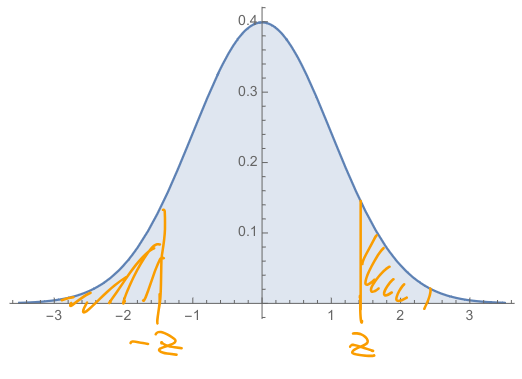
\includegraphics[width=0.7\linewidth]{images/moivrelaplaceGlocke}
    \caption{}\label{fig:moivrelaplaceGlocke}
\end{figure}
\begin{erg} \txc{(2026)}
    \textbf{Lokaler zentraler Grenzwertsatz und Satz von de Moivre-Laplace} \\
    % \texttt{Siehe Folie 25--29}
    % 2026 F 36-40
    \begin{figure}[H]
        \centering
        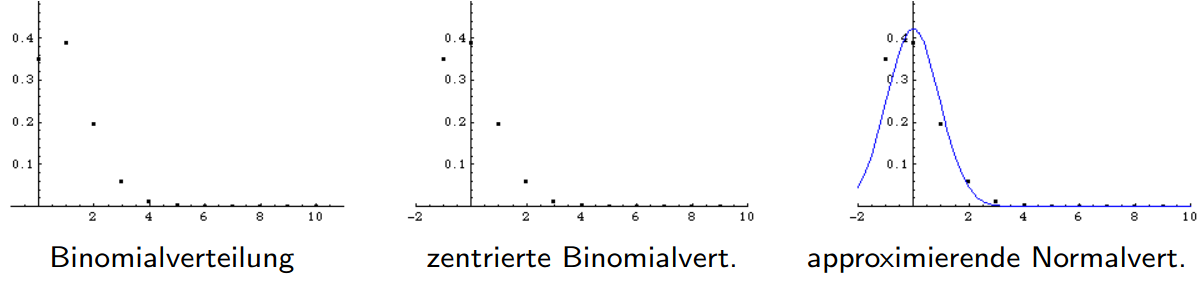
\includegraphics[width=0.7\linewidth]{images/verteilungsgraphenZehn}
        \caption{Beispiel für n = 10, p = 1/10}\label{fig:verteilungsgraphenZehn}
    \end{figure}
    \begin{figure}[H]
        \centering
        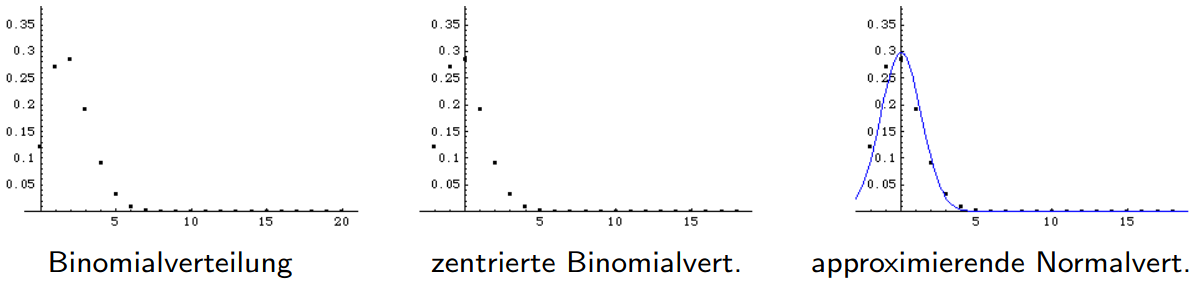
\includegraphics[width=0.7\linewidth]{images/verteilungsgraphenZwanzig}
        \caption{Beispiel für n = 20, p = 1/10}\label{fig:verteilungsgraphenZwanzig}
    \end{figure}
    \begin{figure}[H]
        \centering
        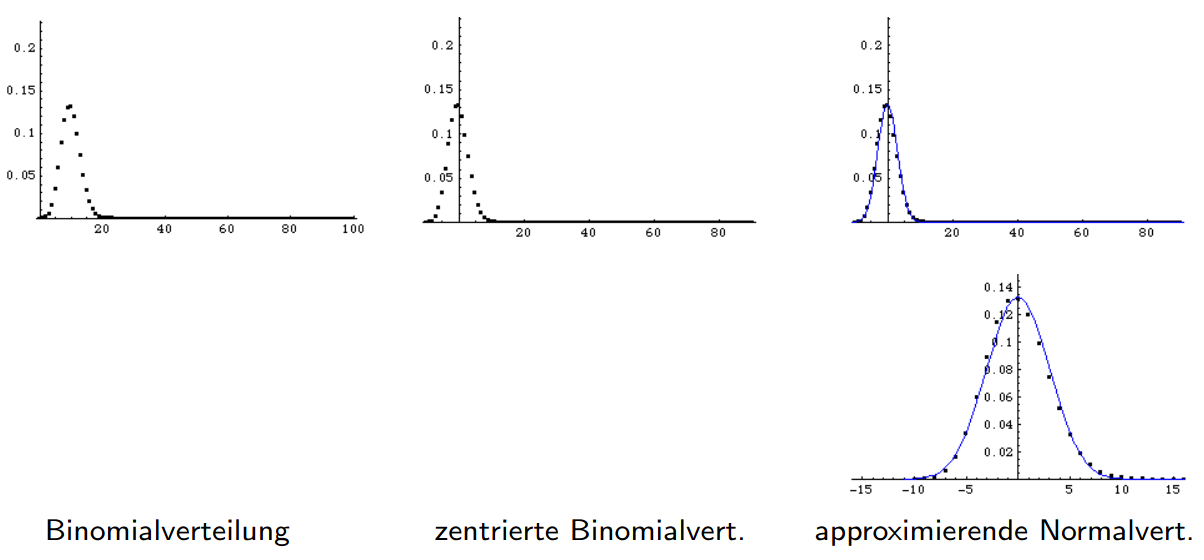
\includegraphics[width=0.7\linewidth]{images/verteilungsgraphenHundert}
        \caption{Beispiel für n = 100, p = 1/10}\label{fig:verteilungsgraphenHundert}
    \end{figure}
    \begin{figure}[H]
        \centering
        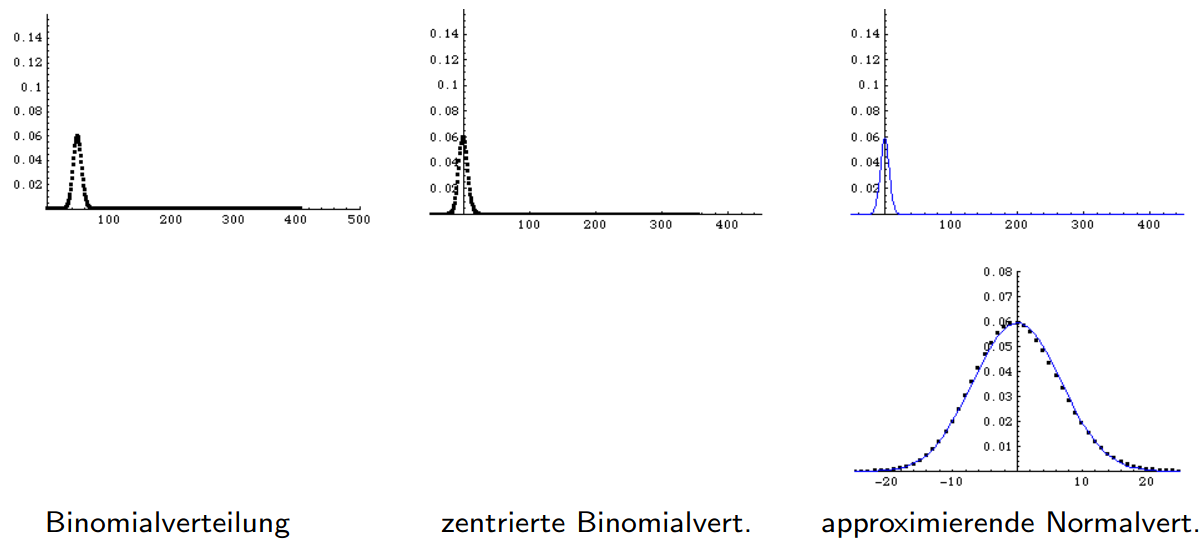
\includegraphics[width=0.7\linewidth]{images/verteilungsgraphenFHundert}
        \caption{Beispiel für n = 500, p = 1/10}\label{fig:verteilungsgraphenFHundert}
    \end{figure}

\end{erg}
\begin{bsp}
    \textbf{Vorlesung vs. Schlaf} \txc{(2025)} \\

    \paragraph{Frage:} Wie groß ist die Wahrscheinlichkeit, dass von den 142 Hörern einer 8-Uhr-Vorlesung nächste Woche zwischen 30\% und 70\% die Vorlesung besuchen?

    \paragraph{Geg.:} \ma{n = 142} Hörer, jeder Einzelne besucht mit Wahrscheinlichkeit \ma{p \in (0,1)} die Vorlesung \ma{(p = \frac{2}{3})}.

    \paragraph{Vereinfachende Annahmen:}
    Alle Hörer besuchen die Vorlesung mit derselben Wahrscheinlichkeit und alle Hörer entscheiden sich unabhängig
    voneinander.

    \paragraph{Modell:} $n$ -mal unabhängig wiederholtes Bernoulli-Experiment mit Erfolgswahrscheinlichkeit $p$.
    Also: Die Anzahl der Erfolge \ma{\sn} ist \ma{\Binomv}-verteilt.
    Man betrachte jeden Anwesenden der n
    eingeschriebenen Hörer als ``Erfolg''. \\
    Also:
    \[
        \glssymbol{eraum} = \kl{0,1}^n, \quad \glssymbol{wfk}(\glssymbol{elementarereignis}) = p^{\sumEN
        \glssymbol{elementarereignis}_i} \cdot (1-p)^{n - \sumEN \glssymbol{elementarereignis}_i}
        \quad (\text{mit } n = 142 \text{ und } p = 2/3)
    \]
    Anzahl der Erfolge ist die Anzahl Anwesender
    \[
        \sn(\glssymbol{elementarereignis}_i) = \sumEN \glssymbol{elementarereignis}_i
    \]
    Dass $n$ Leute anwesende sind, ist das Ereignis:
    \[
        A_n = \kl{\frac{3}{10}\leq \frac{1}{n} \sn  \leq \frac{7}{10}}
        = \{
        \sn \in \{\lceil \frac{3}{10} \cdot n \rceil, \lceil  \frac{3}{10} \cdot n  \rceil + 1, \dots, \lfloor \frac{7}{10} \cdot n \rfloor\}
        \}
    \]
    Für \ma{n = 142} ist das \ma{\lceil \frac{3}{10} \cdot n \rceil = 43} und  \ma{\lfloor \frac{7}{10} \cdot n \rfloor = 99}
    Mit \ma{p =\frac{2}{3}}:
    \[
        \pe(A_n) = \sum_{k = \lceil \frac{3}{10} \cdot n \rceil}^{\lfloor \frac{7}{10} \cdot n \rfloor} \binom{142}{k} \left(\frac{2}{3}\right)^k \left(\frac{1}{3}\right)^{142-k} \txc{ = \sum_{k = 43}^{99} \binom{142}{k} \left(\frac{2}{3}\right)^k \left(\frac{1}{3}\right)^{142-k}}  \approx 0.80
    \]
    Approximation mit dem Satz von de Moivre-Laplace \txo{(in Form $a < \dots \leq b$ bringen)}:
    \begin{align*}
        \pe(A_n) & = \pe(\frac{3n}{10}) \leq \sn \leq \frac{7n}{10} \\
        & \txo{= \pe( \lceil \frac{3n}{10} \rceil  \leq \sn \leq \lfloor \frac{7n}{10} \rfloor)}  \\
        & = \pe(\lceil \frac{3n}{10} \rceil -1  < \sn \leq \lfloor \frac{7n}{10} \rfloor) &
        \text{(weil $\sn$ ganzzahlig ist)} \\
        & = \pe ( a < \frac{\sn - np}{\sqrt{npq}} \leq b ) & \text{(Standardisieren, q = 1 - p = 1/3)} \\
        & \overset{\txo{*}}{\approx} \vfkt(b) - \vfkt(a) & \text{(Satz von de Moivre-Laplace)}\\
        & \approx \vfkt(0.77) - 0 \\
        & \approx 0.7794v & (Tabelle)
    \end{align*}
    \[
        \txo{
            * \intab \varphi(x) \dx = \vfkt(b) - \vfkt(a)
        }
    \]
    mit
    \[
        a = \frac{\lceil \frac{3n}{10} \rceil - 1 - np}{\sqrt{npq}} \approx -9.38 \quad und \quad  b = \frac{\lfloor \frac{7n}{10} \rfloor - 1 - np}{\sqrt{npq}} \approx 0.77
    \]
    % todo \texttt{Mehr Folie 38 bis 45} 2025 ??
\end{bsp}

Das Resultat wirft einige Fragen auf:
\begin{fr}
    \textbf{Warum spielt die untere Grenze a, die von den 30\% herrührt, praktisch keine
    Rolle?} \txc{(2026)}

    \paragraph{1. Antwort:} $\vfkt (a) \approx \vfkt(-9) = 1 - \vfkt(9)$ und $\vfkt(9)$ ist so nah an 1, dass wir diesen
    Wert nicht einmal in der Tabelle finden .
    .
    . \\
    Aber das erklärt noch gar nichts – oder?

    \paragraph{2. Antwort:} Wir wissen aus dem Gesetz der großen Zahlen, dass $\frac{1}{n} \sn$ in einem
    gewissen Sinne gegen $p = 2/3 \approx 66\%$ konvergiert.
    Daher ist die Forderung,
    dass $\frac{1}{n} \sn \leq 70\%$ sein soll, sehr viel restriktiver als die Forderung $\frac{1}{n} \sn \geq 30\%$.
\end{fr}

\komm{Da $\frac{1}{n}\sn$ nach dem Gesetz der großen Zahlen gegen
    $p=\frac{2}{3}\approx 66{, }7\%$ konvergiert, liegt es für große $n$
    mit hoher Wahrscheinlichkeit in der Nähe von $66{, }7\%$. Die Bedingung
    $\frac{1}{n}\sn \ge 30\%$ ist daher nahezu immer erfüllt, während
    $\frac{1}{n}\sn \le 70\%$ nur eine kleine Abweichung vom Grenzwert
    zulässt und somit restriktiver ist.}

\karkar{def_standardisierung_zufallsvariable}
\karkar{satz_moivre_laplace}
\karkar{def_dichte_standardnormalverteilung}
\karkar{def_verteilungsfunktion_standardnormalverteilung}
\karkar{bem_rechenregeln_standardnormalverteilung_grenzwerte}
\karkar{bem_symmetrie_standardnormalverteilung}

\subsection{Anwendungstechniken zum Satz von de Moivre-Laplace}

\begin{fr}
    Die exakte Rechnung ergab $\pe(A_n) \approx 0.80$ (Genauer $\pe(\erga_n) \approx 0.804486$).
    \textbf{Warum finden wir mit dem Satz von de Moivre-Laplace nur $pe(A_n) \approx 0.78$?}
    \txc{(2026)}
    \paragraph{1. Antwort:} n = 142 ist noch kein wirklich großes n.

    \paragraph{2. Antwort:} Grob gesprochen, approximieren wir eine diskrete Größe, die
    Anzahl der Erfolge $\sn$, durch etwas Kontinuierliches.
    Eine Verbesserung ist oft
    möglich durch die sogenannte Stetigkeitskorrektur: \index{Stetigkeitskorrektur}.

    Wir modifizieren die Grenzen in $A_n$ geschickt und rechnen
    \begin{align*}
        \pe(A_n) & = \pe(\lceil \frac{3n}{10} \rceil -1  < \sn \leq \lfloor \frac{7n}{10} \rfloor) \\
        & \pe(\lceil \frac{3n}{10} \rceil \txo{- \frac{1}{2}}  < \sn \leq \lfloor \frac{7n}{10} \rfloor \txo{+
        \frac{1}{2}} ) & \text{(weil $\sn$ ganzzahlig ist)} \\
        & \approx \vfkt(0.86) \approx 0.8051 & (Tabelle)
    \end{align*}
    \txc{Bingo!} \\
    Beachte, dass die Stetigkeitskorrektur nicht immer besser ist (siehe Hausaufgaben).
\end{fr}

\begin{bsp}
    \textbf{Vorlesung vs. Schlaf II} \txc{(2026)} \\

    Wie groß ist die Wahrscheinlichkeit, dass
    von 142 Hörern nächste Woche mindestens
    90 die Vorlesung besuchen?

    \paragraph{Was ist anders als im obigen Beispiel?} Neu an dieser Frage ist, dass wir nur eine untere Schranke gegeben haben,
    d.h., wir suchen die Wahrscheinlichkeit von
    \[
        B_n = \{\sn \geq 90\}
    \]
    Dieser Fall ist in unserer Formulierung des Satzes von de Moivre-Laplace nicht
    vorgesehen!

    \paragraph{Idee, das Problem zu umgehen:} Wir werden uns künstlich eine triviale obere Schranke verschaffen.
    \begin{align*}
        \pe(B_n) & = \pe(\sn \geq 90) \\
        & = \pe(89 < \sn \leq n ) & \text{(triviale obere Schranke)} \\
        & = \pe(89.5 < \sn \leq n ) & (\sn\text{ ganzzahlig, Stetigkeitskorrektur)} \\
        & \pe( c_n < \frac{\sn - np}{\sqrt{npq}} \leq d_n ) & (Standardisieren) \\
        & \approx \vfkt(d_n) - \vfkt(c_n) & \text{(Satz von de Moivre-Laplace)} \\
        & = \vfkt(d_n) - [1- \vfkt( \oub{-c_n}{>0} )] \approx 0.8212 & (Tabelle)
    \end{align*}
    mit \[
            c_n = \frac{89.5 - np}{\sqrt{npq}} \approx -0.92 \quad und \quad d_n = \frac{nq}{\sqrt{npq}} 0 \sqrt{\frac{nq}{p}} \approx 8.43.
    \]
    Exakte Rechnung ergibt $\pe(B_n) = 0.821556 \dots$
\end{bsp}

\begin{bem} \txc{(2026)} \\
    Generell gelten, sofern der Satz von de Moivre-Laplace anwendbar ist,
    \[
        \pe (s_n > c) = \pe\left(
        \frac{c-np}{\sqrt{npq}} < \frac{\sn-np}{\sqrt{npq}} \leq \frac{n-np}{\sqrt{npq}}
        \right) \approx 1 - \vfkt\left(\frac{c-np}{\sqrt{npq}}\right)
    \]
    und
    \[
        \pe (s_n \leq d) = \pe\left(
        \frac{-1-np}{\sqrt{npq}} < \frac{\sn-np}{\sqrt{npq}} \leq \frac{d-np}{\sqrt{npq}}
        \right) \approx \vfkt\left(\frac{d-np}{\sqrt{npq}}\right)
    \]
    weil für große n
    \[
        \vfkt\left(\frac{-1-np}{\sqrt{npq}}\right) \approx 0 \quad und \quad \frac{n-np}{\sqrt{npq}} \approx 1
    \]
\end{bem}

\karkar{bem_technik_ganzzahligkeit_bei_diskretisierung}
\karkar{def_stetigkeitskorrektur}
\karkar{bem_technik_einseitige_schranke_kuenstliche_grenze}
\karkar{bem_allgemeine_formel_obere_grenzwahrscheinlichkeit}
\karkar{bem_allgemeine_formel_untere_grenzwahrscheinlichkeit}
\karkar{bem_interpretation_vernachlaessigbare_grenze}
